\documentclass[12pt]{article}
\usepackage{amsmath,amssymb}
\usepackage{geometry}
\geometry{margin=1in}
\usepackage[hidelinks]{hyperref}
\setlength{\parindent}{0pt}
\usepackage{xcolor}
\usepackage{etoolbox}  %Supports toggle commands
\definecolor{darkblue}{RGB}{0,0,139}
\usepackage{tikz}
\usepackage{pgfplots}
\pgfplotsset{compat=1.18}

%SETTINGS
\newtoggle{solutions} \togglefalse{solutions}

\begin{document}

\begin{center}
\textbf{Problem Set 3} \\
Introduction to Health Economics: EC 387 \\
Boston University \\
Spring 2026 \\
Professor Pauline Mourot
\end{center}

\vspace{1em}

\noindent \textbf{Exercise 1: TRUE/FALSE/UNCERTAIN}\\

For each of the questions below, please explain your answer.
The quality of the explanation is an important part of the grade for these problems and
can also help you earn substantial partial credit.
In answering each question, 1-3 sentences of explanation should be sufficient.

\vspace{7mm}
\noindent \textbf{QUESTION 1}\\
Asymmetric information in insurance markets
(such as when consumers know more about their medical expenditure risks than insurers)
leads to unraveling in insurance markets and uninsured individuals.

\iftoggle{solutions}{
{ \color{darkblue}

\vspace{5mm}

FALSE/UNCERTAIN. 
If risk aversion is strong, the risk premium could be high enough so that all consumers would be willing to buy insurance,
and there would be no unravelling.
Unraveling depends on the extent of adverse selection and risk aversion.
}}{}

\vspace{7mm}

\noindent \textbf{QUESTION 2}\\
A monopolist insurer selling a single insurance contract will choose to sell insurance to everyone
and avoid adverse selection altogether.

\iftoggle{solutions}{
{\color{darkblue}

\vspace{5mm}

FALSE/UNCERTAIN.
A monopolist may still be better off setting a higher price that only the highest cost consumers will purchase.
See the adverse selection slides where we have an example of a monopolist insurer that chooses to only sell insurance to the highest cost consumers,
and not to the lowest cost consumers.

}}{}

\vspace{7mm}

\noindent \textbf{QUESTION 3}\\
In a selection market with imperfect information,
imposing an insurance mandate necessarily decreases the average cost for insurers.

\iftoggle{solutions}{
{\color{darkblue}

\vspace{5mm}

FALSE.
The expected impact of an insurance mandate on the average cost for insurers depends on the
type of selection in the market.
If there is advantageous selection, an insurance mandate would increase the average cost for insurers,
because it would bring in more high-cost consumers.
In the case of adverse selection, an insurance mandate would decrease the average cost for insurers,
because it would bring in more low-cost consumers.
That is what Hackmann, Kolstad, and Kowalski (2015, AER) found in Massachusetts when they implemented an insurance mandate in 2006.

}}{}

\vspace{7mm}

\noindent \textbf{QUESTION 4}\\
The willingness to pay for insurance is always above the marginal cost.

\iftoggle{solutions}{
{\color{darkblue}

\vspace{5mm}

FALSE.
It depends on the individual's risk-profile and risk-preferences.
A risk-averse consumer may have a willingness to pay for insurance that is above the expected medical costs for the insurer,
because they are willing to pay a risk premium to avoid the uncertainty of medical costs.
However, even in the case of risk aversion, this depends on their risk profile.

}}{}

\vspace{7mm}


\noindent \textbf{Exercise 2: A selection market}\\

\medskip

Consider a market with the demand (WTP) and MC curves defined as below.

\begin{center}
\begin{tabular}{c c c c c}
\hline
$Q$ & Individual Cost (MC) & WTP & Total Cost & Average Cost \\
\hline
1 & 10 & 17 &  &  \\
2 & 8  & 13 &  &  \\
3 & 6  & 9  &  &  \\
4 & 4  & 5  &  &  \\
\hline
\end{tabular}
\end{center}

\bigskip
\noindent\textbf{a.} What does MC correspond to in real life?
\medskip

\iftoggle{solutions}{
{ \color{darkblue}

The marginal cost corresponds to the expected medical bills paid by the insurance company for the additional person.

}
}{}

\medskip
\noindent\textbf{b.} Are WTP and MC positively or negatively correlated? Why?
\medskip

\iftoggle{solutions}{
{ \color{darkblue}

They are positively correlated here, because the higher the WTP, the higher the marginal cost in the table.
Why would it be positively correlated? Because if I am sicker, I know I will have higher medical bills,
so I will be willing to pay more for insurance.
}
}{}

\medskip
\noindent\textbf{c.} Fill in the table above for Total Cost and Average Cost.
\medskip

\iftoggle{solutions}{
{

\begin{center}
\begin{tabular}{c c c c c}
\hline
$Q$ & Individual Cost (MC) & WTP & Total Cost & Average Cost \\
\hline
1 & 10 & 17 & {\color{darkblue} 10} & {\color{darkblue} 10} \\
2 & 8  & 13 & {\color{darkblue} 18} & {\color{darkblue} 9} \\
3 & 6  & 9  & {\color{darkblue} 24} & {\color{darkblue} 8} \\
4 & 4  & 5  & {\color{darkblue} 28} & {\color{darkblue} 7} \\
\hline
\end{tabular}
\end{center}

}
}{}

\medskip
\noindent\textbf{d.} Draw the demand curve, the MC curve, and the AC curve in the (Q,P) plane as we saw in class.
\medskip

\iftoggle{solutions}{
{ 
\begin{center}
% Same visual axis length: choose x and y units so 4.8*xunit ≈ 18.2*yunit
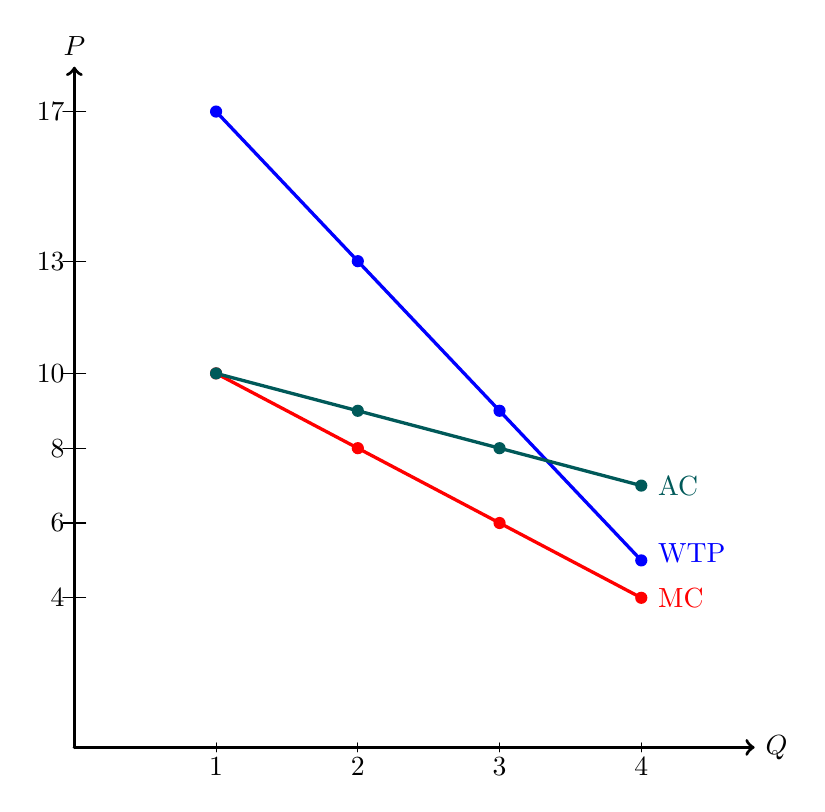
\begin{tikzpicture}[x=1.8cm,y=0.475cm, line cap=round, line join=round]
    % Axes
    \draw[very thick,->] (0,0) -- (4.8,0) node[right] {$Q$};
    \draw[very thick,->] (0,0) -- (0,18.2) node[above] {$P$};

    % X-axis ticks
    \foreach \x in {1,2,3,4}{
        \draw (\x,0.12) -- (\x,-0.12);
        \node[below] at (\x,0) {\x};
    }

    % Y-axis ticks
    \foreach \y in {4,6,8,10,13,17}{
        \draw (0.08,\y) -- (-0.08,\y);
        \node[left] at (0,\y) {\y};
    }

    % Curves
    \draw[blue, very thick] (1,17) -- (2,13) -- (3,9) -- (4,5);            % WTP
    \draw[red, very thick]  (1,10) -- (2,8) -- (3,6) -- (4,4);              % MC
    \draw[teal!70!black, very thick] (1,10) -- (2,9) -- (3,8) -- (4,7);     % AC

    % Points
    \foreach \p in {(1,17),(2,13),(3,9),(4,5)} \fill[blue] \p circle (2.2pt);
    \foreach \p in {(1,10),(2,8),(3,6),(4,4)} \fill[red] \p circle (2.2pt);
    \foreach \p in {(1,10),(2,9),(3,8),(4,7)} \fill[teal!70!black] \p circle (2.2pt);

    % Labels
    \node[blue, right] at (4.05,5.2) {WTP};
    \node[red, right] at (4.05,4.0) {MC};
    \node[teal!70!black, right] at (4.05,7.0) {AC};
\end{tikzpicture}
\end{center}
}
}{}

\vspace{7mm}

\noindent \textbf{Exercise 3: adverse selection and the provision of health insurance}\\

\medskip

Suppose that in each of the insurance markets below, there is adverse selection
(i.e., consumers with higher willingness to pay for insurance are most costly to insure), and
that the markets are perfectly competitive (i.e., insurers make zero profits in equilibrium).

\vspace{3mm}

For each question, draw a demand curve, marginal cost curve, and average cost curve in the (Q,P) plane
such that the markets are consistent with the following (call the total market size $Q^{\text{MAX}}$).
Also explain in a few sentences why your curves are consistent with the statement in the question.

\medskip
\noindent\textbf{a.} At the competitive equilibrium, no insurance is transacted.
\medskip
\iftoggle{solutions}{

{\color{darkblue}

The competitive equilbrium is such that profits are zero, so the price is equal to the average cost.
No insurance is transacted if the average cost curve is above the demand curve at every level of quantity until $Q^{\text{MAX}}$,
so that the demand curve never intersects the average cost curve. 
It would look like this:
}

\begin{center}
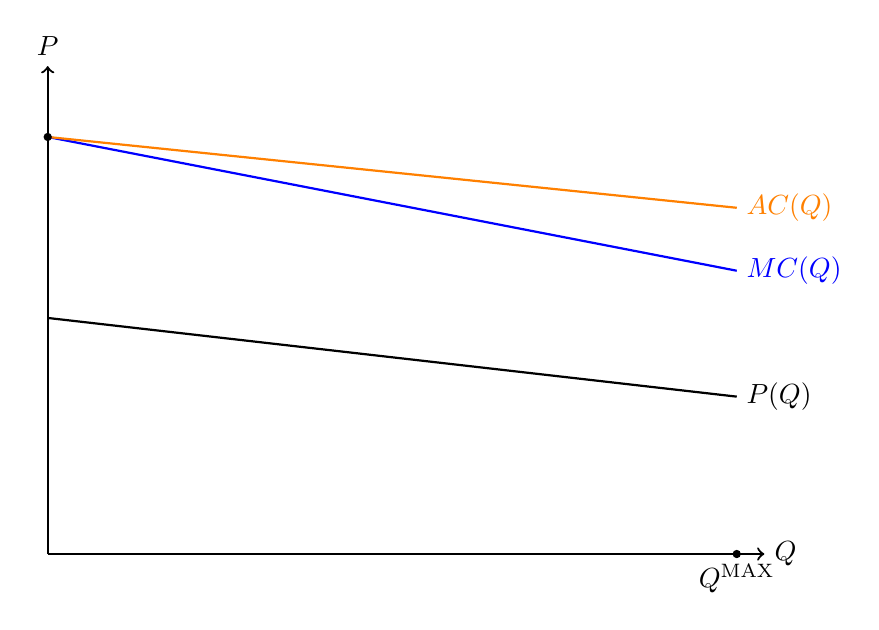
\begin{tikzpicture}[x=0.035cm, y=0.0020cm, scale=0.5]

    % Axes
    \draw[->, thick] (0,0) -- (520,0) node[right] {$Q$};
    \draw[->, thick] (0,0) -- (0,6200) node[above] {$P$};

    % Q^MAX location (where all three curves stop)
    \def\Qmax{500}

    % Curves
    \draw[thick]         (0,3000) -- (\Qmax,2000);   % P(Q)
    \draw[blue, thick]   (0,5300) -- (\Qmax,3600);   % MC(Q)
    \draw[orange, thick] (0,5300) -- (\Qmax,4400);   % AC(Q)

    % Labels to the right of curve ends
    \node[right] at (\Qmax,2000) {$P(Q)$};
    \node[blue, right] at (\Qmax,3600) {$MC(Q)$};
    \node[orange, right] at (\Qmax,4400) {$AC(Q)$};

    % Shared y-intercept marker for MC and AC
    \fill (0,5300) circle[radius=3pt];

    % Mark and label Q^MAX on x-axis
    \fill (\Qmax,0) circle[radius=3pt];
    \node[below] at (\Qmax,0) {$Q^{\text{MAX}}$};

\end{tikzpicture}
\end{center}


}
{}

\medskip
\noindent\textbf{b.} At the competitive equilibrium, everyone in the population is insured.
\medskip
\iftoggle{solutions}{

{\color{darkblue}

Everyone is insured if the demand curve is above the average cost curve and
intersects the average cost curve at $Q^{\text{MAX}}$ or after.
It would look like this:
}

\begin{center}
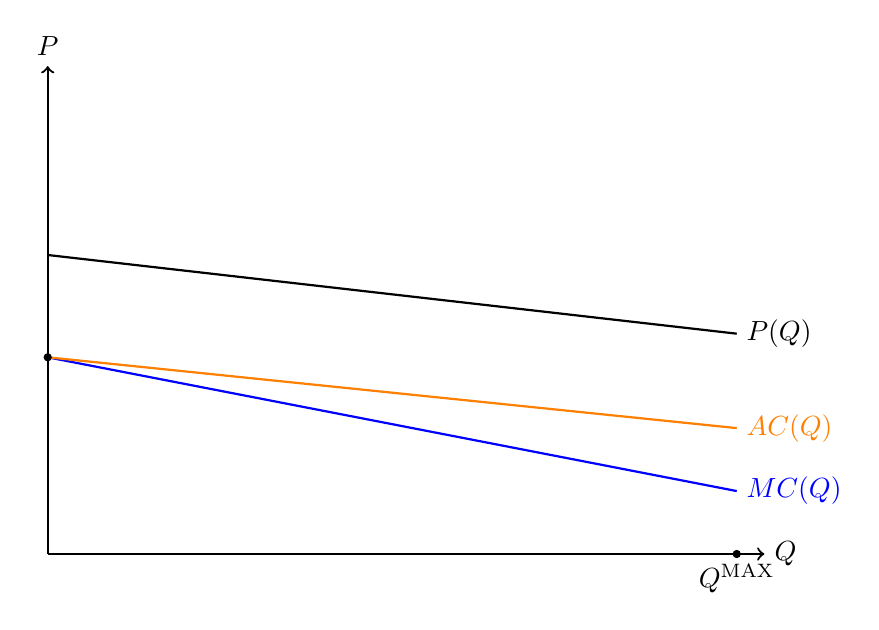
\begin{tikzpicture}[x=0.035cm, y=0.0020cm, scale=0.5]

    % Axes
    \draw[->, thick] (0,0) -- (520,0) node[right] {$Q$};
    \draw[->, thick] (0,0) -- (0,6200) node[above] {$P$};

    % Q^MAX location
    \def\Qmax{500}

    % Demand moved up for clarity
    \draw[thick] (0,3800) -- (\Qmax,2800);  % P(Q)

    % MC and AC keep same slopes as before, translated down
    % MC slope = (3600-5300)/500 = -3.4
    % AC slope = (4400-5300)/500 = -1.8
    \draw[blue, thick]   (0,2500) -- (\Qmax,800);   % MC(Q)
    \draw[orange, thick] (0,2500) -- (\Qmax,1600);  % AC(Q)

    % Labels to the right of curve ends
    \node[right] at (\Qmax,2800) {$P(Q)$};
    \node[blue, right] at (\Qmax,800) {$MC(Q)$};
    \node[orange, right] at (\Qmax,1600) {$AC(Q)$};

    % Shared y-intercept marker for MC and AC
    \fill (0,2500) circle[radius=3pt];

    % Mark and label Q^MAX
    \fill (\Qmax,0) circle[radius=3pt];
    \node[below] at (\Qmax,0) {$Q^{\text{MAX}}$};

\end{tikzpicture}
\end{center}


}
{}

\medskip
\noindent\textbf{c.} At the competitive equilibrium, only half of the population buys insurance.
\medskip
\iftoggle{solutions}{

{\color{darkblue}

Half of the population buys insurance if the demand curve intersects the average cost curve at exactly half of $Q^{\text{MAX}}$.
It would look like this:
}
\begin{center}
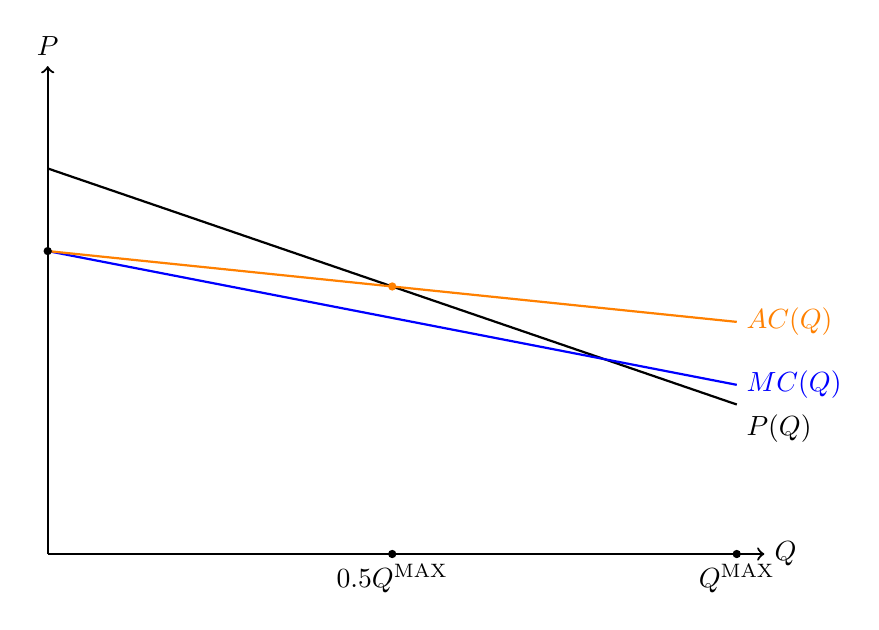
\begin{tikzpicture}[x=0.035cm, y=0.0020cm, scale=0.5]

    % Axes
    \draw[->, thick] (0,0) -- (520,0) node[right] {$Q$};
    \draw[->, thick] (0,0) -- (0,6200) node[above] {$P$};

    % Key x-values
    \def\Qmax{500}
    \def\Qmid{250}

    % Demand: steeper, and still intersects AC at Q = 0.5 Q^MAX
    % Passes through (250,3400), slope = -6  => (0,4900) to (500,1900)
    \draw[thick] (0,4900) -- (\Qmax,1900);           % P(Q)

    % MC and AC (same as before; same y-intercept)
    \draw[blue, thick]   (0,3850) -- (\Qmax,2150);   % MC(Q)
    \draw[orange, thick] (0,3850) -- (\Qmax,2950);   % AC(Q)

    % Labels to the right
    \node[right] at (\Qmax,1600) {$P(Q)$};
    \node[blue, right] at (\Qmax,2150) {$MC(Q)$};
    \node[orange, right] at (\Qmax,2950) {$AC(Q)$};

    % Shared y-intercept marker for AC and MC
    \fill (0,3850) circle[radius=3pt];

    % Mark Q^MAX and 0.5Q^MAX
    \fill (\Qmax,0) circle[radius=3pt];
    \node[below] at (\Qmax,0) {$Q^{\text{MAX}}$};

    \fill (\Qmid,0) circle[radius=3pt];
    \node[below] at (\Qmid,0) {$0.5Q^{\text{MAX}}$};

    % AC = Demand at Q = 0.5Q^MAX
    \fill[orange] (\Qmid,3400) circle[radius=3pt];

\end{tikzpicture}
\end{center}


}
{}

Now, notice that at every level of quantity, there are gains from trade so long as the demand
curve exceeds the marginal cost curve. At any level of
quantity, the vertical distance between the demand curve and marginal cost curve represents
the social surplus that would be generated by that transaction.

\vspace{3mm}

With this in mind, now draw the demand, marginal cost, and average cost curves consistent with the situations described below (call the total market size $Q^{\text{MAX}}$).
Also explain in a few sentences why your curves are consistent with the statement in the question.

\medskip
\noindent\textbf{d.} It is socially efficient for no one to have insurance.
\medskip
\iftoggle{solutions}{

{\color{darkblue}

It is socially efficient for no one to have insurance if
the demand curve is below the marginal cost curve at every level of quantity until $Q^{\text{MAX}}$,
so that there are no gains from trade at any level of quantity.
It would look like this:
}

\begin{center}
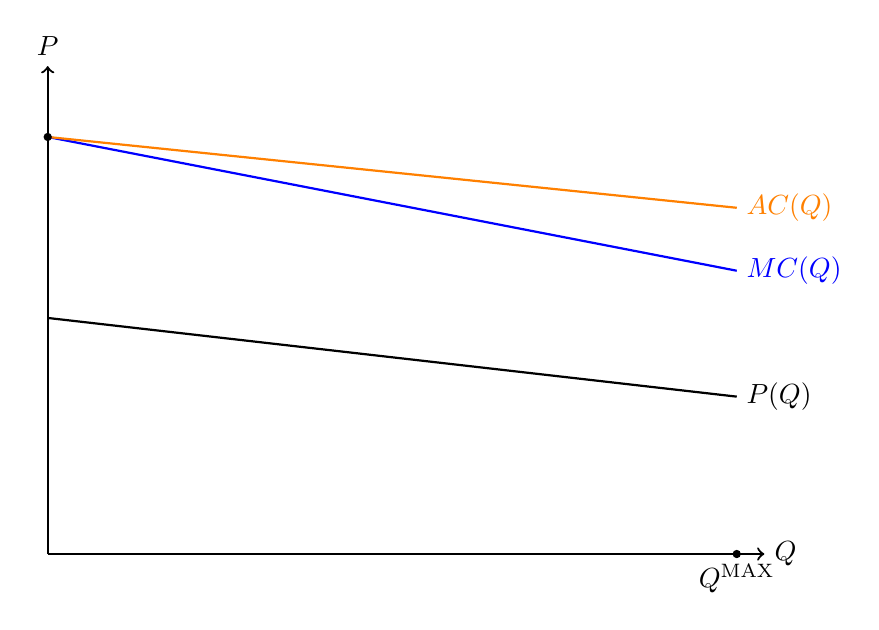
\begin{tikzpicture}[x=0.035cm, y=0.0020cm, scale=0.5]

    % Axes
    \draw[->, thick] (0,0) -- (520,0) node[right] {$Q$};
    \draw[->, thick] (0,0) -- (0,6200) node[above] {$P$};

    % Q^MAX location (where all three curves stop)
    \def\Qmax{500}

    % Curves
    \draw[thick]         (0,3000) -- (\Qmax,2000);   % P(Q)
    \draw[blue, thick]   (0,5300) -- (\Qmax,3600);   % MC(Q)
    \draw[orange, thick] (0,5300) -- (\Qmax,4400);   % AC(Q)

    % Labels to the right of curve ends
    \node[right] at (\Qmax,2000) {$P(Q)$};
    \node[blue, right] at (\Qmax,3600) {$MC(Q)$};
    \node[orange, right] at (\Qmax,4400) {$AC(Q)$};

    % Shared y-intercept marker for MC and AC
    \fill (0,5300) circle[radius=3pt];

    % Mark and label Q^MAX on x-axis
    \fill (\Qmax,0) circle[radius=3pt];
    \node[below] at (\Qmax,0) {$Q^{\text{MAX}}$};

\end{tikzpicture}
\end{center}


}
{}

\medskip
\noindent\textbf{e.} It is socially efficient for everyone to have insurance.
\medskip
\iftoggle{solutions}{

{\color{darkblue}

It is socially efficient for everyone to have insurance if
the demand curve is above the marginal cost curve at every level of quantity until $Q^{\text{MAX}}$,
so that there are gains from trade at every level of quantity.
It would look like this:
}

\begin{center}
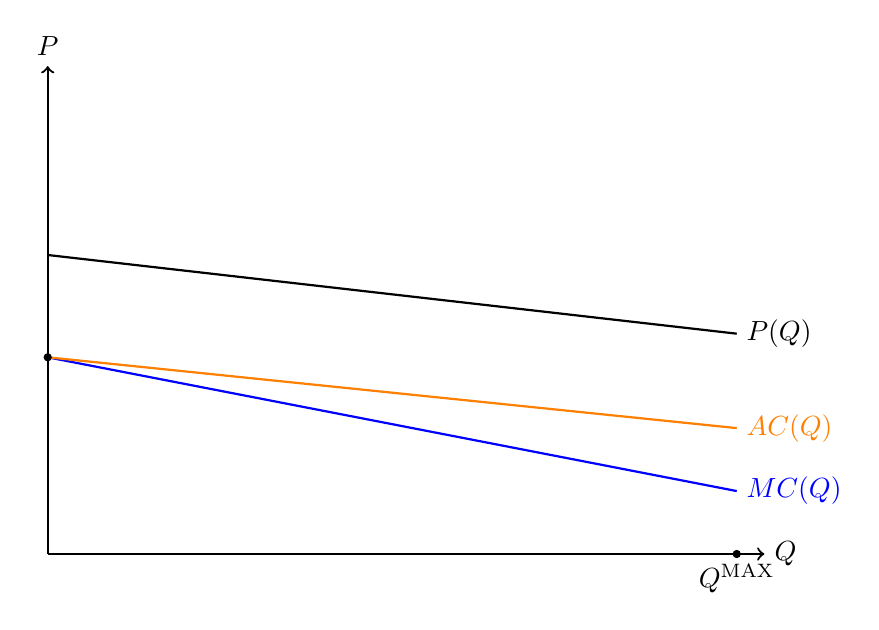
\begin{tikzpicture}[x=0.035cm, y=0.0020cm, scale=0.5]

    % Axes
    \draw[->, thick] (0,0) -- (520,0) node[right] {$Q$};
    \draw[->, thick] (0,0) -- (0,6200) node[above] {$P$};

    % Q^MAX location
    \def\Qmax{500}

    % Demand moved up for clarity
    \draw[thick] (0,3800) -- (\Qmax,2800);  % P(Q)

    % MC and AC keep same slopes as before, translated down
    % MC slope = (3600-5300)/500 = -3.4
    % AC slope = (4400-5300)/500 = -1.8
    \draw[blue, thick]   (0,2500) -- (\Qmax,800);   % MC(Q)
    \draw[orange, thick] (0,2500) -- (\Qmax,1600);  % AC(Q)

    % Labels to the right of curve ends
    \node[right] at (\Qmax,2800) {$P(Q)$};
    \node[blue, right] at (\Qmax,800) {$MC(Q)$};
    \node[orange, right] at (\Qmax,1600) {$AC(Q)$};

    % Shared y-intercept marker for MC and AC
    \fill (0,2500) circle[radius=3pt];

    % Mark and label Q^MAX
    \fill (\Qmax,0) circle[radius=3pt];
    \node[below] at (\Qmax,0) {$Q^{\text{MAX}}$};

\end{tikzpicture}
\end{center}

}
{}

\medskip
\noindent\textbf{f.} It is socially efficient for only half of the population to have insurance.
\medskip
\iftoggle{solutions}{

{\color{darkblue}

It is socially efficient for only half of the population to have insurance if
the demand curve intersects the marginal cost curve at exactly half of $Q^{\text{MAX}}$.
It would look like this:
}

\begin{center}
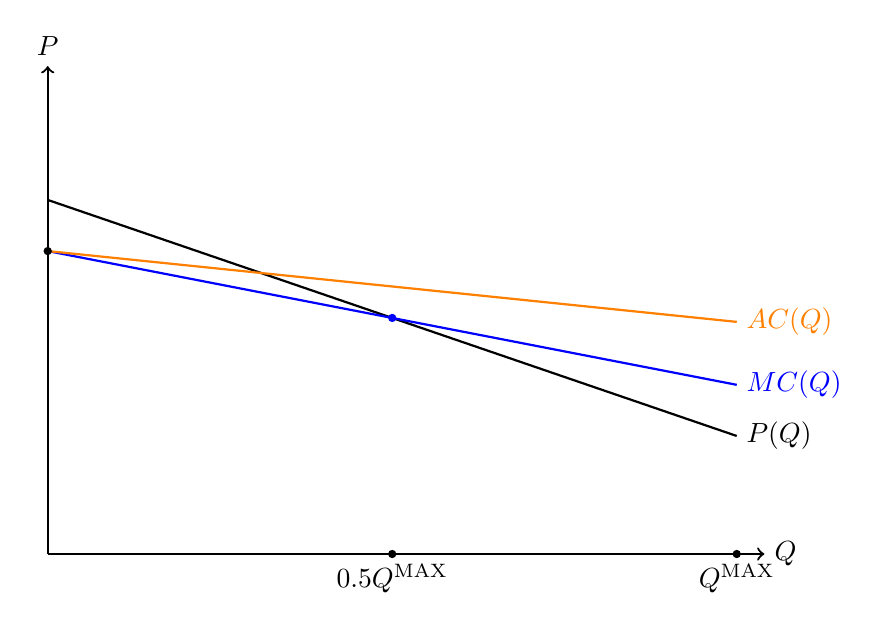
\begin{tikzpicture}[x=0.035cm, y=0.0020cm, scale=0.5]

    % Axes
    \draw[->, thick] (0,0) -- (520,0) node[right] {$Q$};
    \draw[->, thick] (0,0) -- (0,6200) node[above] {$P$};

    % Key x-values
    \def\Qmax{500}
    \def\Qmid{250}

    % Demand: intersects MC at Q = 0.5 Q^MAX
    % Through (250,3000), slope -6 -> (0,4500) to (500,1500)
    \draw[thick] (0,4500) -- (\Qmax,1500);           % P(Q)

    % MC and AC (same as before; same y-intercept)
    \draw[blue, thick]   (0,3850) -- (\Qmax,2150);   % MC(Q)
    \draw[orange, thick] (0,3850) -- (\Qmax,2950);   % AC(Q)

    % Labels to the right
    \node[right] at (\Qmax,1500) {$P(Q)$};
    \node[blue, right] at (\Qmax,2150) {$MC(Q)$};
    \node[orange, right] at (\Qmax,2950) {$AC(Q)$};

    % Shared y-intercept marker for AC and MC
    \fill (0,3850) circle[radius=3pt];

    % Mark Q^MAX and 0.5Q^MAX
    \fill (\Qmax,0) circle[radius=3pt];
    \node[below] at (\Qmax,0) {$Q^{\text{MAX}}$};

    \fill (\Qmid,0) circle[radius=3pt];
    \node[below] at (\Qmid,0) {$0.5Q^{\text{MAX}}$};

    % Demand = MC at Q = 0.5Q^MAX
    \fill[blue] (\Qmid,3000) circle[radius=3pt];

\end{tikzpicture}
\end{center}

}
{}


\end{document}